\documentclass[12pt,a4paper]{article}
\usepackage[utf8]{inputenc} 
\usepackage[T1]{fontenc}		       
\usepackage{lmodern}			       
\usepackage{babel} 
\usepackage{amsmath}
\usepackage{amsfonts}
\usepackage{amssymb}
\usepackage{graphicx}
\usepackage{xcolor}
\usepackage{mathtools}
\usepackage{fancyhdr}
\usepackage{enumitem}
\usepackage{tcolorbox}
\usepackage{stmaryrd}
\usepackage{dsfont}
\usepackage{pgf, tikz}
\usetikzlibrary{shapes.misc}
\usepackage[linesnumbered,ruled,vlined]{algorithm2e}
\usepackage[text={15cm,24.5cm},centering]{geometry}

% Définir le texte affiché en fin de page
\pagestyle{fancy}
\fancyhf{}  % Clear the default headers and footers
\rfoot{\hrule
    \vspace{0.3cm}
    \noindent\textsf{Félix de Brandois}
    \hfill \thepage
}
\renewcommand{\headrulewidth}{0pt}

% Style de l'entete
\newcommand{\entete}{
    \noindent\textbf{INSA - ModIA, 4$^e$ année.}
    \hfill \textbf{Années 2023-2024}
    
    \begin{center}
        \textbf{\LARGE Machine Learning}
    \end{center}
}


% Définir la fonction pour créer une boîte de propriété
\newcommand{\propriete}[2]{%
    \begin{tcolorbox}[colback=white,colframe=green!25!white,title=\textbf{Propriété #1}, coltitle=black]
        #2
    \end{tcolorbox}
}

% Définir la fonction pour créer une boîte de définition
\newcommand{\definition}[2]{%
    \begin{tcolorbox}[colback=white,colframe=blue!25!white,title=\textbf{Définition #1}, coltitle=black]
        #2
    \end{tcolorbox}
}

% Définir la fonction pour créer une boîte de théorème
\newcommand{\theoreme}[2]{%
    \begin{tcolorbox}[colback=white,colframe=red!25!white,title=\textbf{Théorème #1}, coltitle=black]
        #2
    \end{tcolorbox}
}

% Définir la fonction pour créer une boîte de remarque
\definecolor{customRed}{RGB}{150, 30, 30}
\newcommand{\remarque}[1]{%
    \leftline{\noindent
    \textcolor{customRed}{\vrule width 3pt}\hspace{10pt}%
    \parbox{0.9\textwidth}{%
        \textbf{Remarque :}
        #1
    }}
    \vspace{10pt}
}

% Définir la fonction pour créer une boîte de preuve
\newcommand{\preuve}[1]{%
    \begin{quote}
        $\blacktriangleright$~#1
    \end{quote}
}

% Définir la fonction pour créer un encadrement de texte
\newcommand{\important}[1]{%
    \begin{tcolorbox}[colback=red!10!white,colframe=red!30!black]
        #1
    \end{tcolorbox}
}



\begin{document}

\entete

\vspace{0.5cm}

\part{Bases du Machine Learning}

\section{Notations}

\begin{tcolorbox}[colback=white,colframe=blue!50!white]
    \begin{itemize}
        \item $\mathcal{X}$ : espace des entrées.
        \item $\mathcal{Y}$ : espace des sorties (exemples : $\{-1, 1\}$, $\mathbb{R}$).
        \item $S = \{(x_i, y_i)\}_{1 \leq i \leq m}$.
        \item $h : \mathcal{X} \longrightarrow \mathcal{Y}$ : modèle de prédiction.
        \item $\mathcal{H}$ : ensemble des modèles de prédiction.
        \item $L : \mathcal{H} \times (\mathcal{X} \times \mathcal{Y}) \longrightarrow \mathbb{R}$ : fonction de perte.
        \item \
        \begin{array}[t]{lrcl}
            R_D : & \mathcal{H} & \longrightarrow & \mathbb{R} \qquad \text{risque empirique} \\
                & h & \longmapsto & \mathbb{E}_{(x, y) \sim D} [L(h(x), y)]
        \end{array}
    \end{itemize}
\end{tcolorbox}

\noindent\textbf{Exemples :}
\begin{itemize}
    \item $L(h(x), y) = \mathds{1}_{h(x) \neq y}$, $R_D(h) = \mathbb{P}_{(x, y) \sim D} [h(x) \neq y]$.
    \item $L(h(x), y) = (h(x) - y)^2$, $R_D(h) = \mathbb{E}_{(x, y) \sim D} [(h(x) - y)^2]$.
\end{itemize}


\important{
    \begin{equation}
        h_S = \underset{h \in \mathcal{H}}{\text{argmin }} \hat{R}_S(h) \quad \text{avec} \quad \hat{R}_S(h) \text{ estimateur de } R_D(h)
    \end{equation}
}

\underline{Comment analyser $R_D(\hat{h}_S)$ ?}

\section{Courbes ROC}

\begin{tcolorbox}[colback=white,colframe=blue!50!white]
    \begin{itemize}
        \item $h_S$ : seuil score.
        \item score : $\mathcal{X} \longrightarrow \mathbb{R}$.
        \item \
        \begin{array}[t]{lrcl}
            \text{seuil} : & \mathbb{R} & \longrightarrow & \mathcal{Y} \\
                & x & \longmapsto & \begin{cases}
                    1 & \text{si } x < \mu \\
                    -1 & \text{si } x \geq \mu
                \end{cases}
        \end{array}
    \end{itemize}
\end{tcolorbox}

\noindent\textbf{Exemple :}\\

\begin{tabular}{| l | c | c | c | c | c | c |}
    \hline
    x & $x_1$ & $x_2$ & $x_3$ & $x_4$ & $x_5$ & $x_6$ \\
    \hline
    y & 1 & -1 & 1 & 1 & -1 & -1 \\
    \hline
    score(x) & 0.99 & 0.95 & 0.51 & 0.45 & 0.10 & 0.01 \\
    \hline
\end{tabular}

\definition{- Sensibilité et spécificité}{
    On pose : $\mathcal{T}^+ = \{(x_i, y_i) \in S \text{ tels que } y_i = 1\}$\\
    et : $\mathcal{T}^- = \{(x_i, y_i) \in S \text{ tels que } y_i = -1\}$ \\

    Sensibilité : $\frac{1}{|\mathcal{T}^+|} \sum_{(x_i, y_i) \in \mathcal{T}^+} \mathds{1}_{h_S(x_i) = 1}$\\
    Spécificité : $\frac{1}{|\mathcal{T}^-|} \sum_{(x_i, y_i) \in \mathcal{T}^-} \mathds{1}_{h_S(x_i) = -1}$
}

\remarque{
    \begin{itemize}
        \item Sensibilité : taux de vrais positifs.
        \item Spécificité : taux de vrais négatifs.
    \end{itemize}
}

\remarque{
    \\Anti-spécificité (ou taux de faux positifs) : $\frac{1}{|\mathcal{T}^-|} \sum_{(x_i, y_i) \in \mathcal{T}^-} \mathds{1}_{h_S(x_i) = 1}$
}

\noindent\textbf{Exemple :}\\

\begin{tabular}{| l | c | c | c | c | c | c |}
    \hline
    $\mu$ & $> 0.99$ & $]0.95, 0.99]$ & $]0.51, 0.95]$ & $]0.45, 0.51]$ & $]0.10, 0.45]$ & $]0.01, 0.10]$ \\
    \hline
    Sensibilité & $0$ & $1/3$ & $1/3$ & $2/3$ & $1$ & $1$ \\
    \hline
    Anti-spécificité & $0$ & $0$ & $1/3$ & $1/3$ & $1/3$ & $2/3$ \\
    \hline
\end{tabular}

\vspace{0.5cm}

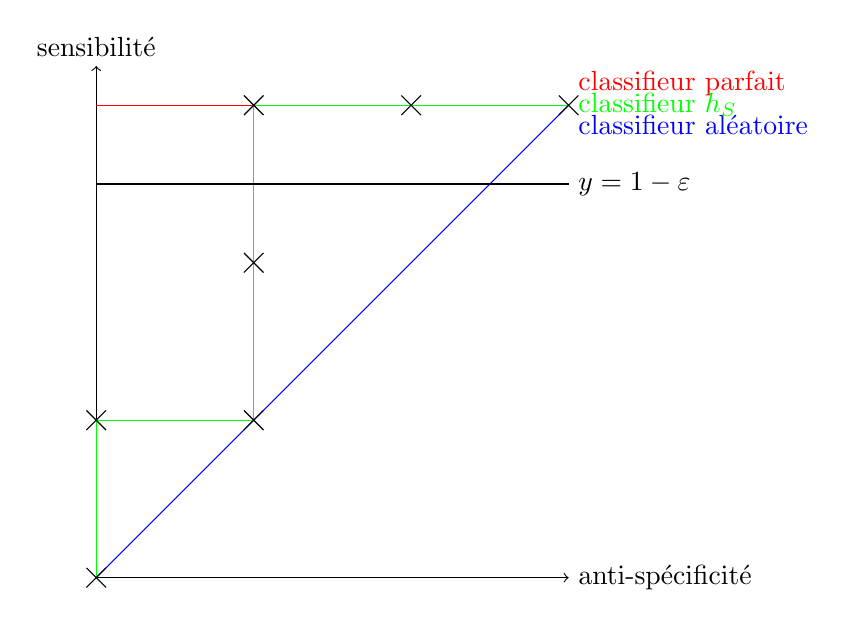
\begin{tikzpicture}
    \draw[->] (0,0) -- (6,0) node[right] {anti-spécificité};
    \draw[->] (0,0) -- (0,6.5) node[above] {sensibilité};
    \draw[red] (0,6) -- (6,6) node[above right] {classifieur parfait};
    \draw[blue] (0,0) -- (6,6) node[below right] {classifieur aléatoire};
    \draw[green] (0,0) -- (0,2) -- (2,2) -- (2,6) -- (6,6) node[right] {classifieur $h_S$};
    \draw (0,0) node[cross out, draw] {};
    \draw (0,2) node[cross out, draw] {};
    \draw (2,2) node[cross out, draw] {};
    \draw (2,4) node[cross out, draw] {};
    \draw (2,6) node[cross out, draw] {};
    \draw (4,6) node[cross out, draw] {};
    \draw (6,6) node[cross out, draw] {};
    \draw (0,5)  -- (6,5) node[right] {$y = 1 - \varepsilon$};
\end{tikzpicture}


Aire sous la courbe :
\begin{itemize}
    \item $\text{AUC}_{\text{classifieur parfait}} = 1$.
    \item $\text{AUC}_{\text{classifieur aléatoire}} = 0.5$.
    \item $\text{AUC}_{h_S} = 7/9$.
\end{itemize}




\end{document}